\chapter{Results}
\label{Chapter5}
\section{Results}
A baseline model was constructed. This model looked at the gust factor for some training data and took the average of this and predicted this average everytime. Several baseline guesses were created based on a lower limit assigned to the average wind speed limit (AWSL). As the average wind speed increases, then the variability in gust as a percentage decreases\cite{mean_gust_HA_HO}. This means looking at a subset of the data where the AWSL is higher, a better result can be expected. The results show this. Several different AWSL were used for the baseline model, as can be seen in table \ref{table:results}. This sets a goal. A model that does not significantly improve on this baseline suggests either failure to capture essential patterns in the data or that the data itself may lack the necessary information for substantial improvements upon the baseline. Using the previously described neural network architecture setups for each AWSL, with and without landscape elevation information, MAPE was determined. The results can be seen in Table \ref{table:results}.

\begin{table}[h]
    \caption[Model results for different AWSL]{MAPE for each average wind speed limit with and without landscape elevation in a 30°sector around the point of interest into the direction of the reanalysis wind. The percentage error is higher for lower wind speeds and thus observing the error for different lower bound of wind speed will produce different results. How to determine this lower bound can done by measurements (f) or reanalysis wind speed at 15 m/s ($ws_{15}$). The influence of adding elevation data seems to reduce the error.}
    \label{table:results}
    \centering
    \begin{tabular}{c|cccccc}
        \textbf{AWSL} & \textbf{MAPE} & & & & &\\ 
        m/s & Baseline & &  Without elevation & & With elevation & \\
            & $ws_{15}$ & f & $ws_{15}$ & f & $ws_{15}$ & f\\\hline
        0 & 39.2\% & 39.2\% & 19.7\% & 15.9\% & 18.6\% & 15.3\%\\
        5 & 28.1\% & 14.8\% & 15.9\% & 9.9\% & 14.1\% & 9.4\%\\
        7.5 & 25.3\% & 12.6\% & 14.5\% & 8.6\% & 12.5\% & 8.6\%\\
        10 & 23.9\% & 11.1\%& 13.6\% & 7.6\% & 11.5\% & 7.4\%\\
        12.5 & 23.3\% & 10.1\% & 13.1\% & 7.1\% & 11.0\% & 6.9\%\\
        15 & 23.2\% & 9.3\% & 13.0 & 7.0\% & 10.6\% & 6.4\%\\
        17.5 & 23.7\% & 8.7\% & 12.8\% & 6.4\% & 10.53\% & 6.1\%\\
        20 & 24.7\% & 8.2\% & 13.6\% & 6.3\% & 11.1\% & 5.8\%\\
        22.5 & 26.1\% & 7.8\% & 14.5\% & 6.1\% & 12.6\% & 5.7\%\\
        25 & 27.7\% & 7.3\% & 15.7\% & 5.8\% & 12.9\% & 5.5\% \\
    \end{tabular}
\end{table}

This is some improvement upon the baseline error, with a decrease in error from 23.9\% to 1.8\% depending on the setup used. The power generated by wind mill increases with wind speed cubed\cite{wind_power}. The highest wind gusts in Iceland are around 70 m/s. Knowing the gust factor to 2 percentage points better than before can allow for the anticipated power generated by wind mills to increase significantly.

\section{Discussion}
The error improvement is modest in absolute terms but represents at least 1.8\% over the baseline. Looking only at the error, the performance of the model can be gauged. However it does not help us explain why the model made these predictions. Here feature interpretation can be of great help. Using Shapley values and the python SHAP package, the contribution of each attribute can be given a value, as previously mentioned. Figure \ref{fig:ShapleyWaterfall} shows the contribution of each feature for a given example.

\begin{figure}[h]
    \centering
    \caption[Feature importance for a single observation of a neural network.]{Feature importance of a neural network with model architecture as described in table \ref{table:gridSearchHyperparamters} and data as described in table \ref{table:trainDataExample}. In this specific instance the wind direction ($wd_15$) has the highest negative influence and the temperature has the highest positive influence. Elevation data is excluded when working with Shapley values, as the contribution of each elevation point is very low and there are very many of them. To see their influence on the model output see Table \ref{table:results}.}
    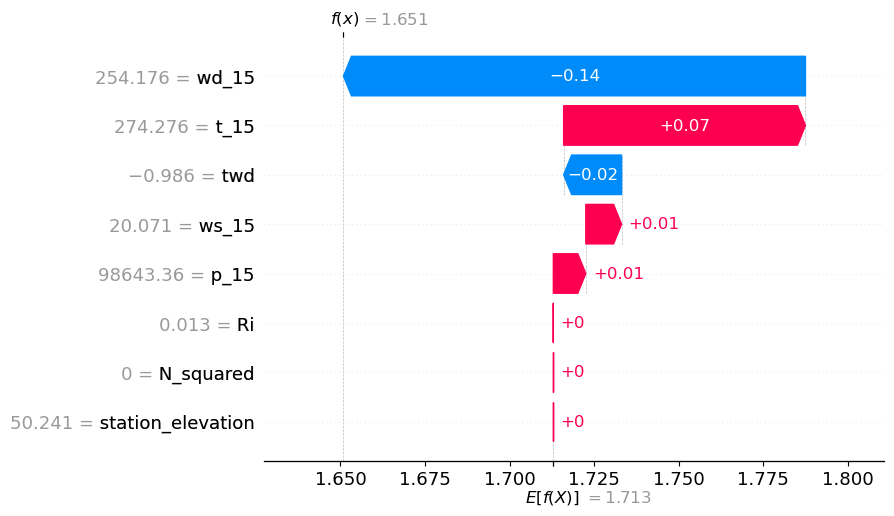
\includegraphics[scale = 0.6]{Figures/waterfall_plot.png}
    \label{fig:ShapleyWaterfall}
\end{figure}

In Figure (\ref{fig:ShapleySummary}) the contribution of each feature, excluding the elevation points, can be seen for the model in general (a significant subset of data is used).

\begin{figure}
    \centering
    \caption[Feature importance of a neural network.]{Feature importance of a neural network with model architecture as described in table \ref{table:gridSearchHyperparamters} and data as described in table \ref{table:trainDataExample}. We can see that generally multiple factors influence the prediction, with the station elevation being highly influential. There is seemingly one outlier for the Richardson number, which usually has very little influence. Elevation data is excluded when working with Shapley values, as the contribution of each elevation point is very low and there are very many of them. To see their influence on the model output see Table \ref{table:results}.}
    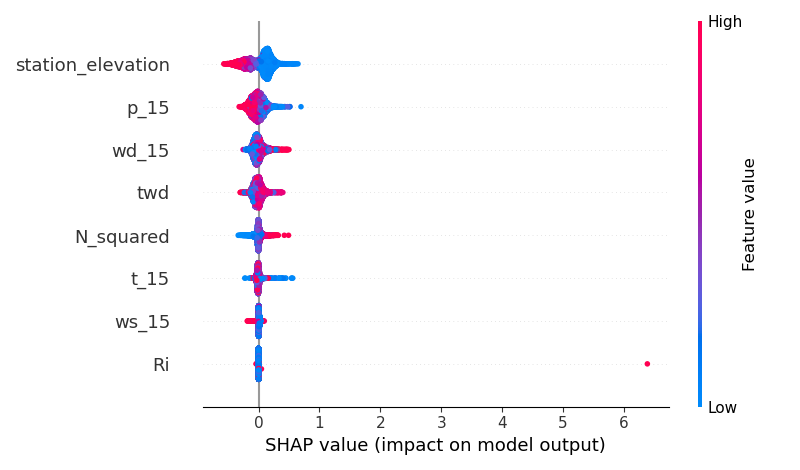
\includegraphics[scale = 0.6]{Figures/summary_plot.png}
    \label{fig:ShapleySummary}
\end{figure}